\documentclass[coverpage,lineno]{../custom}
\usepackage[dvipsnames,table]{xcolor}
\usepackage{tabularx}
\usepackage{multicol}
\usepackage{multirow}
\usepackage{makecell}
\usepackage{pdflscape}
\usepackage{pgfgantt}
\usepackage{tikz}
\usepackage{ctable}
\usepackage{listings}
\usepackage[style=numeric-comp,alldates=iso]{biblatex}
\usetikzlibrary{arrows.meta}
\renewcommand{\cellalign}{lc}
\newcolumntype{L}[1]{>{\hsize=#1\hsize\raggedright\arraybackslash}X}
\newcolumntype{C}[1]{>{\hsize=#1\hsize\arraybackslash}X}
\newcolumntype{R}[1]{>{\hsize=#1\hsize\raggedleft\arraybackslash}X}
\definecolor{RedOrange}{RGB}{255,83,0}

\addbibresource{../references.bib}

\newcommand{\musthave}{{\color{red}Must have}}
\newcommand{\shouldhave}{{\color{orange}Should have}}
\newcommand{\couldhave}{{\color{Green}Could have}}
\usepackage{longtable}
\usepackage{boldline}
\usepackage{everypage}

\newcommand{\FunctionalReq}[8]{
\begin{longtable}{|p{0.225\textwidth}|p{0.725\textwidth}|}
\hline
	\textbf{ID - Name} & \textbf{#1 - #2} \\\hlineB{2}
	\textbf{Description} & #3 \\\hline
	\textbf{\makecell*{Priority - {\color{red}Mu\color{orange}Sh\color{Green}Co}}} & #4
	
	#5 \\\hline
	\textbf{Dependencies} & #6 \\\hline
	\textbf{Expected Results} & #7 \\\hline
	\textbf{Exception handling} & #8 \\\hline
\end{longtable}
}
\newcommand{\NonFunctionalReq}[7]{
\begin{longtable}{|p{0.155\textwidth}|p{0.795\textwidth}|}
	\hline
	\textbf{ID - Name} & \textbf{#1 - #2} \\\hlineB{2}
	\textbf{Type} & #3 \\\hline
	\textbf{Priority} & #4 \\\hline
	\textbf{Description} & #5 \\\hline
	\textbf{Metrics} & #6 \\\hline
	\textbf{Constraints} & #7 \\\hline
\end{longtable}

}
\newcommand{\NonFunctionalReqSec}[8]{
\begin{longtable}{|p{0.155\textwidth}|p{0.795\textwidth}|}
	\hline
	\textbf{ID - Name} & \textbf{#1 - #2} \\\hlineB{2}
	\textbf{Type} & #3 \\\hline
	\textbf{Priority} & #4 \\\hline
	\textbf{Description} & #5 \\\hline
	\textbf{Metrics} & #6 \\\hline
	\textbf{Constraints} & #7 \\\hline
\end{longtable}
}
\newcommand{\Risk}[4]{
\begin{longtable}{|p{0.125\textwidth}|p{0.825\textwidth}|}
	\hline
	\textbf{ID - Risk} & \textbf{\makecell*{#1 - #2}} \\\hlineB{2}
	\textbf{Risk} & #3 \\\hline
	\textbf{Mitigation} & #4 \\\hline
\end{longtable}
}
\newcommand{\RiskMatrix}[9]{
\begin{tabularx}{\textwidth}{C{0.15}C{0.65}|L{1.4}|L{1.4}|L{1.4}|}
	\cline{3-5}
	& & \multicolumn{3}{c|}{\textbf{Impact}} \\\cline{3-5}
	& & \makecell*{Low} & \makecell*{Medium} & \makecell*{High}\\\hline
	\multicolumn{1}{|c}{\multirow{3}{*}{\rotatebox[origin=c]{90}{\textbf{Probability }}}} & \multicolumn{1}{|l|}{Unlikely} & \cellcolor{Green}\makecell*{#1} & \cellcolor{LimeGreen}\makecell*{#2} & \cellcolor{YellowOrange}\makecell*{#3} \\\cline{2-5}
	\multicolumn{1}{|c}{} & \multicolumn{1}{|l|}{Possible} & \cellcolor{LimeGreen}\makecell*{#4} & \cellcolor{YellowOrange}\makecell*{#5} & \cellcolor{RedOrange}\makecell*{#6} \\\cline{2-5}
	\multicolumn{1}{|c}{} & \multicolumn{1}{|l|}{Likely} & \cellcolor{YellowOrange}\makecell*{#7} & \cellcolor{RedOrange}\makecell*{#8} & \cellcolor{Red}\makecell*{#9} \\\hline
\end{tabularx}

}

\newcommand{\Lpagenumber}{\ifdim\textwidth=\linewidth\else\bgroup
  \dimendef\margin=0 %use \margin instead of \dimen0
  \ifodd\value{page}\margin=\oddsidemargin
  \else\margin=\evensidemargin
  \fi
  \raisebox{\dimexpr -\topmargin-\headheight-\headsep-0.5\linewidth}[0pt][0pt]{%
    \rlap{\hspace{\dimexpr \margin+\textheight+\footskip}%
    \llap{\rotatebox{90}{\thepage}}}}%
\egroup\fi}
\AddEverypageHook{\Lpagenumber}%

\Title{Requirement Specification}

\begin{document}
\pagenumbering{gobble}
\maketitle
\tableofcontents\newpage
\pagenumbering{arabic}


\section{Introduction}
\label{sec:intro}

\subsection{Overview and Justification}
\label{ssec:just}

This document provides the requirement specifications for our virtual reality (VR) meditation application, referred to henceforth as `the product'; the specific software for the product shall be referred to as `the software'. This document provides an introduction (\cref{sec:intro}) to the project, covering the justification (\cref{ssec:just}), scope (\cref{ssec:scope}), and systems (\cref{ssec:desc}); the requirements for the system (\cref{sec:req}), both functional (\cref{ssec:f_req}) and non-functional (\cref{ssec:nf_req}), and potential risks and issues (\cref{ssec:risks}); the development of the project (\cref{sec:dev}) in terms of the approach (\cref{ssec:dev_approach}) and schedule (\cref{ssec:schedule}).

This project is for Professor Alexandra Cristea who shall henceforth be referred to as 'the client'. The client has given us the project of developing a VR meditation application with the possible use as a basis for research into the topic. This project aims to help those who have not done any, or have done very little, meditation before by giving them an immersive VR world to aid concentration and relaxation.

\subsection{Project Scope}
\label{ssec:scope}

This project is intended for those who have never done any, or done very little, meditation before. It is aimed primarily at adults. The app is intended to help with mindfulness meditation (MM) practice through the use of gamification concepts and VR. The primary objectives are as follows:

\begin{itemize}
	\item Personalisation over customisation\\
	The client would prefer for the project to personalise, that is automatic adjustments to suit the user, itself rather than have the user customise the project, that is allowing the user to alter the environment
	\item Stability\\
	The client would prefer fewer stable features over more less-stable features
	\item Modularity\\
	The client would prefer the software to be modular to allow for ease of reuse in future projects
\end{itemize}

The client would also like the potential to use the project later on in a research context. This is not a primary consideration of ours, but we will use this to guide our development. To ensure that our project can be as seamlessly used in this context with little impact on the project itself, we will make reference to relevant literature where necessary to ensure our implementations of MM is as concurrent with current literature as we can make it\footnote{The authors can find little research on MM with VR implementations. There is a significant amounts of research into VR applications and MM separately which we will use to guide our development}.

For some examples of literature we will likely make reference of, see \cite{kosunen_relaworld_2016, tang_neuroscience_2015, wang_reducing_2022}. We will also make significant reference to \cite{lan_slow_2021} as a good example of research into a similar topic.

\subsection{System Description}
\label{ssec:desc}

The system will be a VR app intended for meditation with aspects of gamification\cite{toda_taxonomy_2019} using the Meta Quest\footnote{Previously Oculus Quest}. The app is intended to aid with visualisation based meditation and to accelerate the progression through meditation training.

The primary section of the app will be set in an environment designed to have as little distraction as possible whilst still allowing the app to be engaging. At present, we intend for the environment to be relatively featureless, with some objects orbiting the user. The objects will themselves have particles around them to obfuscate any highly contrasting areas. Each session will be approximately 10 to 20 minutes in length and various metrics will be measured throughout such as heart rate, EEG data, and eye tracking. This will be analysed and stored externally in accordance with the GDPR.

Evaluation metrics will be applied to the raw data, the results of which will be used to compare sessions and measure improvement. These metrics will be user-specific and will require user-specific baseline data, as well as general data. To gather this baseline data, a short (at most 5 minutes) baseline session will be required before the user can complete any meditation.

The data metrics will be constructed to account for global limits and will be personalised, via user-specific data, to ensure that any change can be measured relatively to the user and not to some global standard. With this we aim to ensure that all users can see a clear progression from session to session.

Each user will have an associated account that will communicate with the server. This account will contain the user's name and personalisation data. The user will be able to access a history of sessions via a request to the server.

The server itself will be run by a Python script that can be run on any computer. For the purpose of product demonstration, we will ensure the same computer runs both the server and Quest app in lieu of a server with a static IP. The server will store user account data, raw session data, and session metric results. Data will be stored in a XML format, with each user having a folder under their username, with sessions and user data within that folder. Current, incomplete, XML DTD are given in \cref{apdx:xml_dtd}.

\subsubsection{Current systems}

There exists several current systems for integrating VR into meditation. We will briefly discuss two of these such systems here.

Lan et al. \cite{lan_slow_2021} demonstrated a feasible study for multimodal feedback meditation in VR. They used g-tummo meditation which has some well researched benefits \cite{kozhevnikov_neurocognitive_2013} but is a fairly advanced technique. As such the multimodal feedback system allows less experienced meditators to feel a more immediate feedback from meditation and thus attempt to help motivate people to continue meditation. This research showed that the multimodal feedback correlated with a decrease in breathing rate and helped maintain user attention, measured via tiredness.

Hølledig et al. \cite{holledig_zenvr_2018} demonstrated a VR based meditation environment also using biofeedback. Their environment was a generated forest environment with different amounts of fog depending on real-time evaluation of the user's meditative state. Whilst they failed to show any meaningful benefits, they do note that the use of biofeedback has potential to be useful. The authors also note of significant issue with the Myndplay headband that resulted in having to redesign their tests.

\section{Solution Requirements}
\label{sec:req}

\subsection{Functional Requirements}
\label{ssec:f_req}

\begin{figure}[h!]
	\centering
	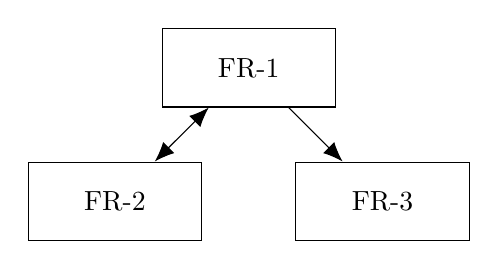
\begin{tikzpicture}[
		node distance=17mm,
		node/.style={rectangle, draw=black, minimum width=22mm, minimum height=10mm}
	]
		\node[node](fr-1){FR-1};
		\node[node](fr-2)[below of=fr-1,xshift=-17mm]{FR-2};
		\node[node](fr-3)[below of=fr-1,xshift=17mm]{FR-3};
		
		\draw[{Latex[length=2.5mm,width=2mm]}-{Latex[length=2.5mm,width=2mm]}](fr-1) -- (fr-2);
		\draw[-{Latex[length=2.5mm,width=2mm]}](fr-1) -- (fr-3);
	\end{tikzpicture}
	\caption{Functional dependency graph}
\end{figure}

\FunctionalReq
{FR-S-1}{Stability}
{Description\\Over multiple lines}
{Priority - \musthave \shouldhave \couldhave}
{No dependencies}
{Results}
{let it all crash}

\subsection{Non-functional Requirements}
\label{ssec:nf_req}

\begin{figure}[h!]
	\centering
	\begin{tikzpicture}[
		node distance=17mm,
		node/.style={rectangle, draw=black, minimum width=22mm, minimum height=10mm}
	]
		\node[node](nfr-1){NFR-1};
		\node[node](nfr-2)[below of=fr-1,xshift=-17mm]{NFR-2};
		\node[node](nfr-3)[below of=fr-1,xshift=17mm]{NFR-3};
		
		\draw[{Latex[length=2.5mm,width=2mm]}-{Latex[length=2.5mm,width=2mm]}](nfr-1) -- (nfr-2);
		\draw[-{Latex[length=2.5mm,width=2mm]}](nfr-1) -- (nfr-3);
	\end{tikzpicture}
	\caption{Non-functional dependency graph}
\end{figure}

\NonFunctionalReq
{NFR-O-1}{Modularity}
{Description\\Over multiple lines}
{No dependencies}
{Priority}
{Metrics}
{Constraints}

\NonFunctionalReqS
{NFR-S-1}{Modularity}
{Description\\Over multiple lines}
{No dependencies}
{Priority}
{Metrics}
{Constraints}
{Security}

\subsection{Risks and Issues}
\label{ssec:risks}

\subsubsection{Risk Matrix}

\RiskMatrix
{r1\\test}{r2}{r3}
{r4}{r5\\test}{r6}
{r7}{r8}{r9\\test}

\section{Project Development}
\label{sec:dev}

\subsection{Development Approach}
\label{ssec:dev_approach}
For our Software Engineering Project, we have decided that an agile approach, specifically Extreme Programming (XP), fits our needs the best. It ensures that we can work on multiple tasks simultaneously and stipulates thorough planning and collaboration, which is inline with our concept

\subsubsection{Advantages of Extreme Programming}
\begin{itemize}
    \item Extensive planning \\
    As detailed in our Project Schedule, our approach has to rely significantly on prior planning and communication. Each piece of code / assessment is meticulously divided into smaller sub-tasks and evaluated based on its length and difficulty. Additionally, the group always confers with the client first to make sure the vision of client till matches the production code.
    \item Pair programming \\
    Two people from the group focus solely on the actual development of the software / code and cross check each other's work. 
    \item Simple design \\
    After meeting whit the client, its has become clear that the data is the primary focus of this project. Personalisation (the collection of data and the subsequent adapting of the meditation) is will be the goal of this project, rather than creating a customizable environment, e.g. prioritizing eye tracking over more colors the user can choose from at the beginning of the meditation. This follows the principle of simple design, since we will focus on raw data collection rather than "bells and whistles".
    \item Refactoring and continuous integration \\
     During the primary development phase outlined in \cref{ssec:schedule} we will have to adapt and refactor the code multiple times for adjustment. This could be due to technical limitations and feedback given in the feedback stage in \cref{ssec:schedule}. Since the client has requested the code be as clean and understandable as possible due to the fact that it might be used for further research later, we will periodically refactor and simplify the code. This will happen frequently, since we are not experienced with VR or C-sharp.
\end{itemize}
\subsubsection{Disadvantages of other methods}
\begin{itemize}
    \item Waterfall \\
    The Waterfall method does not offer the flexibility we need to manage this project in the given time frame. Implementing new requirements or coding practices is virtually impossible because everything has to stick to a rigid schedule. Dividing the workload would also not work with this method. In contrast, the XP method allows for more dynamic workflows and and reflects a realistic relationship with the client
    \item SCRUM \\
    SCRUM has fixed, predefined roles which we feel are not suited for our project. Since we decide everything together and everyone cross checks everyone, there is no need for a SCRUM Master or a product owner. Additionally, the frequency of meetings and the general time spent on a sprint does not coincide with our project schedule. In contrast, XP does not have a predefined time strucutre and does not have hierarchical structures.   
    
    
\end{itemize}

\subsection{Project Schedule}
\label{ssec:schedule}

\Cref{fig:schedule} illustrates our timeline for the duration of this project. The Gantt chart is split into two parts: The actual developing stages of the software/code and the completion of the assessments themselves. 
\subsubsection{Code}
For the software we the phases have familiarisation with the VR-Headsets and C-sharp, the development of the code, feedback from users, testers and the client and minor adjustments in accordance with the provided feedback. Two people will always be working on solely writing the code. 
\subsubsection{Assessments}
Since we have opted for a modular code and work approach, each piece of work we submit is extensively planned and reviewed:
\begin{itemize}
    \item During the 3-5 days before we start on the assessment we divided up the work and discuss key targets
    \item Over the next few weeks each person completes their part of the project, while continuously communicating to other members of the group their progress and if they need advice
    \item When everyone has completed their work, one person reviews every section to help ensure proper spelling, formatting and that every section meets / exceeds expectations
    \item The revision period does not necessarily only mean revising the actual material. It also means reflecting on the work submitted and figuring out how to improve our collaboration process
\end{itemize}

\newgeometry{a4paper,total={155mm,265mm}}
\begin{landscape}
\begin{figure}
\centering
\begin{ganttchart}[
	x unit=0.1cm,
	y unit chart=0.5cm,
	hgrid={black!25},
	link bulge=3,
	time slot format=isodate,
	vrule/.style={very thick, blue}
]{2022-10-08}{2023-04-29}
	\gantttitlecalendar{year, month=name}\\
	\gantttitle{Familiarization}{33}\gantttitle{Primary Development}{72}\gantttitle{Feedback}{20}\gantttitle{Adjustment}{19}\gantttitle{Presentation and Review}{60}

    % req spec
    \ganttgroup[group/.append style={draw=black, fill=red!90!black}]{Requirement Specification}{2022-10-17}{2022-11-15}\\
    \ganttbar[name=req_spec_pre, bar/.append style={fill=red}]{Initial Deliberation}{2022-10-17}{2022-10-21}\\
    \ganttbar[name=req_spec, bar/.append style={fill=red}]{Requirement Specification}{2022-10-21}{2022-11-10}\\
    \ganttbar[name=req_spec_rev, bar/.append style={fill=red}]{Revision}{2022-11-11}{2022-11-15}\\
    \ganttlink{req_spec_pre}{req_spec}
    \ganttlink{req_spec}{req_spec_rev}
    
    % design video pres.
    \ganttgroup[group/.append style={draw=black, fill=green!90!black}]{Design Video Presentation}{2022-11-04}{2022-12-06}\\
    \ganttbar[name=design_video_pre, bar/.append style={fill=green}]{Initial Deliberation}{2022-11-04}{2022-11-08}\\
    \ganttbar[name=design_video, bar/.append style={fill=green}]{Design Video Presentation}{2022-11-08}{2022-12-01}\\
    \ganttbar[name=design_video_rev, bar/.append style={fill=green}  
    ]{Revision}{2022-12-02}{2022-12-06}\\
	\ganttlink[link type=dr]{req_spec}{design_video_pre}
    \ganttlink{design_video_pre}{design_video}
    \ganttlink{design_video}{design_video_rev}
    
    % test plan report
    \ganttgroup[group/.append style={draw=black, fill=yellow!90!black}]{Test Plan Report}{2022-11-24}{2023-01-30} \\
    \ganttbar[name=test_plan_rep_pre,bar/.append style={fill=yellow}]{Initial Deliberation}{2022-11-24}{2022-11-28}\\
    \ganttbar[name=test_plan_rep,bar/.append style={fill=yellow}]{Test Plan Report}{2022-11-28}{2023-01-26}\\
    \ganttbar[name=test_plan_rep_rev, bar/.append style={fill=yellow}]{Revision}{2023-01-27}{2023-01-30}\\
	\ganttlink[link type=dr]{design_video}{test_plan_rep_pre}
    \ganttlink{test_plan_rep_pre}{test_plan_rep}
    \ganttlink{test_plan_rep}{test_plan_rep_rev}
    
    % user manual
    \ganttgroup[group/.append style={draw=black, fill=blue!90!black}]{User Manual}{2023-01-19}{2023-03-13}\\
    \ganttbar[name=user_manual_pre, bar/.append style={fill=blue}]{Initial Deliberation}{2023-01-19}{2023-01-23}\\
    \ganttbar[name=user_manual, bar/.append style={fill=blue}]{User Manual}{2023-01-23}{2023-03-09}\\
    \ganttbar[name=user_manual_rev, bar/.append style={fill=blue}]{Revision}{2023-03-09}{2023-03-13}\\
	\ganttlink[link type=dr]{design_video}{user_manual_pre}
    \ganttlink{user_manual_pre}{user_manual}
    \ganttlink{user_manual}{user_manual_rev}
    
    % product pres.
    \ganttgroup[group/.append style={draw=black, fill=orange!90!black}]{Product Presentation}{2023-02-11}{2023-03-13}\\
    \ganttbar[name=product_pres_pre, bar/.append style={fill=orange}]{Initial Deliberation}{2023-02-11}{2023-02-15}\\
    \ganttbar[name=product_pres, bar/.append style={fill=orange}]{Product Presentation}{2023-02-15}{2023-03-09}\\
    \ganttbar[name=product_pres_rev, bar/.append style={fill=orange}]{Revision}{2023-03-10}{2023-03-13}\\
    \ganttlink{product_pres_pre}{product_pres}
    \ganttlink{product_pres}{product_pres_rev}
    
    % reflective rep
    \ganttbar[name=reflective_rep, bar/.append style={fill=Thistle}]{Reflective Report}{2023-01-30}{2023-04-29}
    \ganttvrule[vrule/.append style={red, ultra thick},vrule label node/.append style={anchor=north east}]{Product Handover}{2023-04-27}
\end{ganttchart}
\caption{Project Schedule Gantt Chart}
\label{fig:schedule}
\end{figure}
\end{landscape}
\restoregeometry

\appendix
\section{XML DTD}
\label{apdx:xml_dtd}

This appendix includes the document type definitions (DTD) for the user and session databases. Each DTD is semi-commented to describe the intended purpose of the given tag or attribute. Due to the project not being complete, the DTD are partially incomplete and the complete parts are best estimates. Any unknown section in the DTDs will be indicated by an ellipsis.

\begin{lstlisting}[language=XML,caption={General DTD for user database}]
<?xml version="1.0"?>
<!DOCTYPE user [
<!ELEMENT user (name, pers_data)>
<!ATTLIST user id ID #REQUIRED>
<!-- User name string -->
<!ELEMENT name (#PCDATA)>
<!-- User personal data -->
<!ELEMENT pers_data (...)>
]>
\end{lstlisting}

\begin{lstlisting}[language=XML,caption={General DTD for session database}]
<?xml version="1.0"?>
<!DOCTYPE session [
<!ELEMENT session (time, HR_data, EEG_data, gaze)>
<!ATTLIST session id ID #REQUIRED>
<!-- Date and time stored as epoch time -->
<!ELEMENT time (#PCDATA)>
<!-- Hear rate data as a list of datapoints -->
<!ELEMENT HR_data ((...)+)>
<!-- EEG data as a list of datapoints -->
<!ELEMENT EEG_data ((...)+)>
<!-- Gaze data as a list of timed datapoints -->
<!ELEMENT gaze ((gaze_element)+)>
<!ELEMENT gaze_element (yaw, pitch)>
<!-- Yaw of the user view -->
<!ELEMENT yaw (#PCDATA)>
<!-- Pitch of the user view -->
<!ELEMENT pitch (#PCDATA)>
<!ATTLIST gaze_element time CDATA #REQUIRED>
]>
\end{lstlisting}

Note that for the child nodes of \texttt{HR\_data} and \texttt{EEG\_data} in the session DTD, each will have a time attribute as with the gaze datapoint.


\begin{lstlisting}[language=XML,caption={Sample session XML file}]
<?xml version = "1.0" encoding = "UTF-8" standalone = "no" ?>
<!DOCTYPE session SYSTEM "session.dtd">
<session id="session id">
	<time>1668110361</time>
	<pers_data>
		...
	</pers_data>
</user>
\end{lstlisting}

\printbibliography

\end{document}


